\section{Media Management example: upload element}
\label{sec:XPR_exmpl_b}

An example of a vertical component is the one that manages media upload on. By introducing a few tags it is possible to handle all the behaviour of the component. In upload case, there is need of only two elements: \texttt{api-upload} and \texttt{part-upload}.
The first one manages the upload functions: server communications and file sending; the second element is a visualization element that shows the input file box and the button ``Choose File''.


The element named \texttt{api-upload} has been designed to upload new files to LocalStorage.
\begin{lstlisting}[language=javascript]
<api-upload id="upload" folder="{{folder}}"
	file="{{file}}" file-name="{{fileName}}">
</api-upload>
\end{lstlisting} 


The element named \texttt{part-upload} has been developed to allow to users to upload new files to LocalStorage.

\begin{lstlisting}[language=javascript]
<api-upload id="upload"
      file="{{file}}" file-name="{{fileName}}">
</api-upload>

<input id="input" type="file" on-change="on_change">
on_change: function () {
      var file = this.$.input.files[0];
      if (!file) {
        return;
      }
      this.fileName = this.fileName || file.name;
      this.file = file;
    }

\end{lstlisting}

The first tag, \texttt{<api-upload>}, set the upload API that handles the request to S3.
The input tag creates a input form that let the user choice the file to upload and trigger the \texttt{on change} function, that send the file via \texttt{<api-upload>} element.



\begin {figure}[h]
\graphicspath{{images/chapter_s3/}}
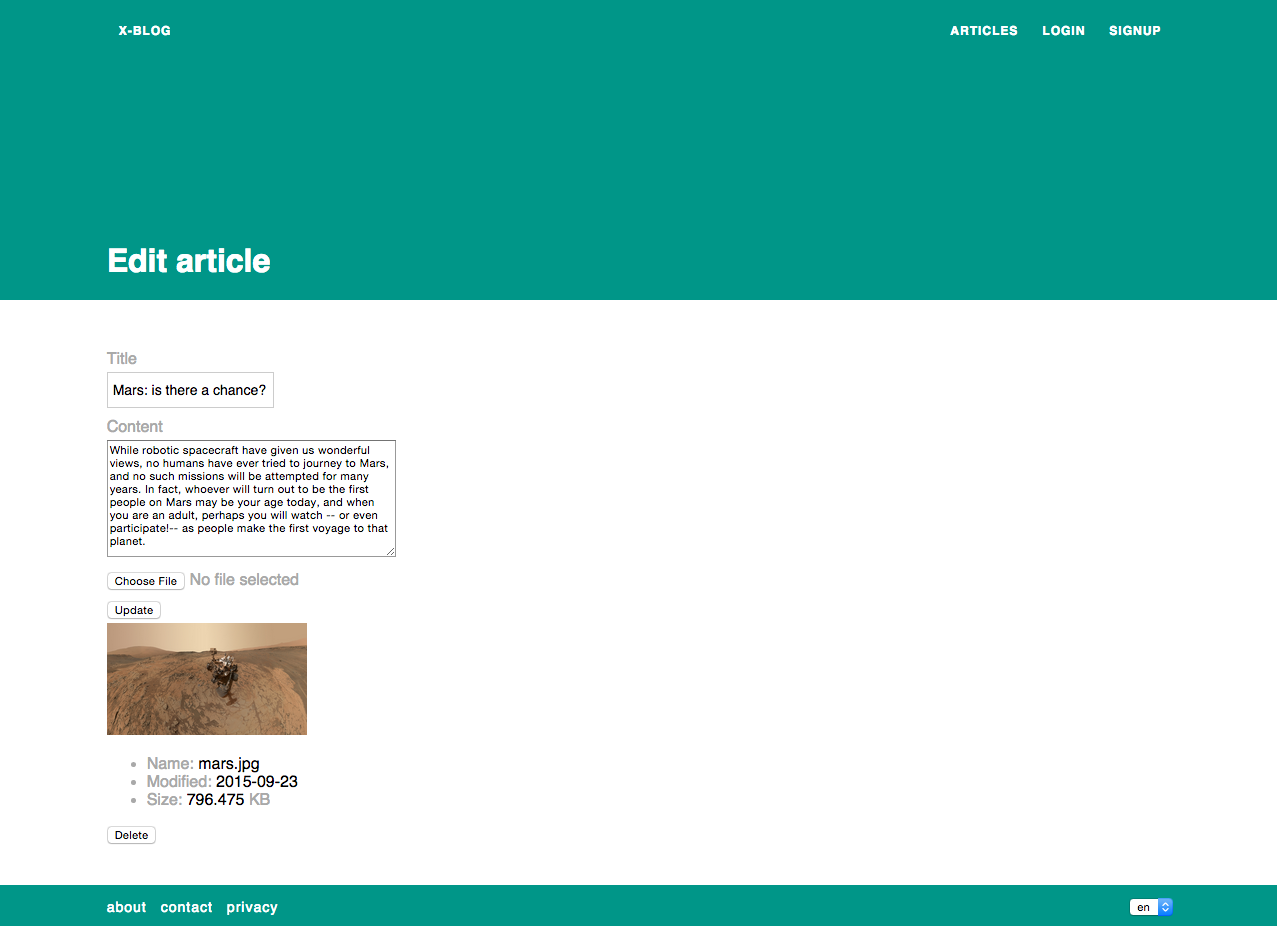
\includegraphics[width=\textwidth]{s3_example}
\caption{Upload component example}
\end {figure}
